\documentclass{standalone}
\usepackage{tikz}
\usepackage{ctex,siunitx}
\setCJKmainfont{Noto Serif CJK SC}
\usepackage{tkz-euclide}
\usepackage{amsmath}
\usetikzlibrary{patterns, calc,3d}
\usetikzlibrary {decorations.pathmorphing,decorations.pathreplacing,decorations.shapes}
\tikzset{label style/.append style={font=\small}}
\begin{document}
\small
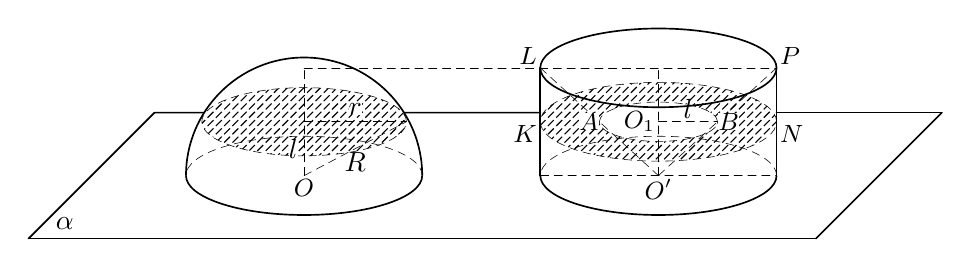
\begin{tikzpicture}[>=latex,scale=1.0,inner sep=1pt]
  \tkzDefPoints{0/0/C,10/0/D,11.6/1.6/E,1.6/1.6/F}
  \tkzDefPoints{3.5/0.8/O,8/0.8/O',5/0.8/rr,2/0.8/rl,3.5/2.1684/rt}
  \tkzDefPoints{9.5/0.8/P',6.5/0.8/L',9.5/1.6/Jr,6.5/1.6/Jl}
  \tkzInterLC(E,F)(O,rl)\tkzGetPoints{Ir}{Il}
  \tkzDefMidPoint(O,rt)\tkzGetPoint{O3}
  \tkzDefShiftPoint[O3](1.299,0){T}
  \tkzDefPointsBy[translation=from O to O3](L',P',O'){K,N,O1}
  \tkzDefPointsBy[translation=from O to rt](L',P',O'){L,P,O2}
  \tkzDefMidPoint(L,O')\tkzGetPoint{A}
  \tkzDefMidPoint(P,O')\tkzGetPoint{B}
  
  \draw[densely dashed,very thin,pattern=north east lines,even odd rule](O1)ellipse(1.5 and 0.5)(O1)ellipse(0.75 and 0.25);
  \tkzDrawSegments[semithick](C,D E,D F,C E,Jr Jl,Ir F,Il P,P' L,L')
  \tkzDrawSegments[densely dashed](O,rt rt,P L',P' L,O' O',P O',O2 O1,B O3,T O,T)
  \draw[semithick](rr)arc(0:-180:1.5 and 0.5);
  \draw[densely dashed,very thin,pattern=north east lines](O3)ellipse({0.75*sqrt(3)} and {0.25*sqrt(3)});
  \draw[very thin,densely dashed](rr)arc(0:180:1.5 and 0.5);
  \draw[semithick](P')arc(0:-180:1.5 and 0.5);
  \draw[very thin,densely dashed](P')arc(0:180:1.5 and 0.5);
  \draw[semithick](O2)ellipse(1.5 and 0.5);
  \tkzDrawArc[semithick](O,rr)(rl)
  \tkzLabelPoints[below](O,O')
  \tkzLabelPoints[above left](L)
  \tkzLabelPoints[below left](K)
  \tkzLabelPoints[above right](P)
  \tkzLabelPoints[below right](N)
  \tkzLabelPoints[right,fill=white,inner sep=0pt](B)
  \tkzLabelPoints[left,fill=white,inner sep=0pt](A)
  \tkzLabelPoint[left](O1){$O_1$}
  \tkzLabelLine[pos=0.5,above](O1,B){$l$}
  \tkzLabelLine[pos=0.5,below](O,T){$R$}
  \tkzLabelLine[pos=0.5,above=2pt,fill=white,inner sep=0pt](O3,T){$r$}
  \tkzLabelLine[pos=0.5,left=2pt,fill=white,inner sep=0pt](O3,O){$l$}
  \tkzLabelAngle[pos=0.5](D,C,F){$\alpha$}
\end{tikzpicture}
\end{document}